\section{Introduction}
\label{sec:introduction}

Wavetable oscillators store one period of a waveform and advance a read pointer modulo the table length.
If $x[0]\neq x[L-1]$, the wrap is a hard discontinuity. Under cyclic playback it becomes a periodic click whose spectrum is broadband and locked to the fundamental.
The same geometry appears whenever a short loop buffer is tiled for listening or for objective evaluation.
We call the repair task \emph{cycle-local seam restoration}: edit a neighborhood of the wrap (and optionally a lightweight residual cell over the period) so that multi-period playback matches an ideal reference that never opens the wrap cliff.
That outer agreement is scored by the prolonged residual $R$ for this periodic seam artifact class.

Figure~\ref{fig:intro-sine} shows one real sine-wrap edge case from the frozen canonical holdout (same \texttt{make\_batch} tile, seed $20{,}260{,}719$).
Panel (a) is the ideal multi-period sine.
Panel (b) is the cracked engine tile after open-wrap cliff modulation ($R\approx0.950$), with the ideal overlaid so the seam jump is visible.
Panel (c) applies DualCosine on that same tile ($R\approx0.603$ on this severe cliff).
Panel (d) is the top DenoiseOpt favorite (\texttt{champion\_iter\_000235}, batch $R\approx0.991$) on the same tile ($R\approx0.9917$).
Panels (e)--(f) plot the modulation residual and a seam zoom so the favorite's correction is readable against DualCosine.

\begin{figure*}[t]
  \centering
  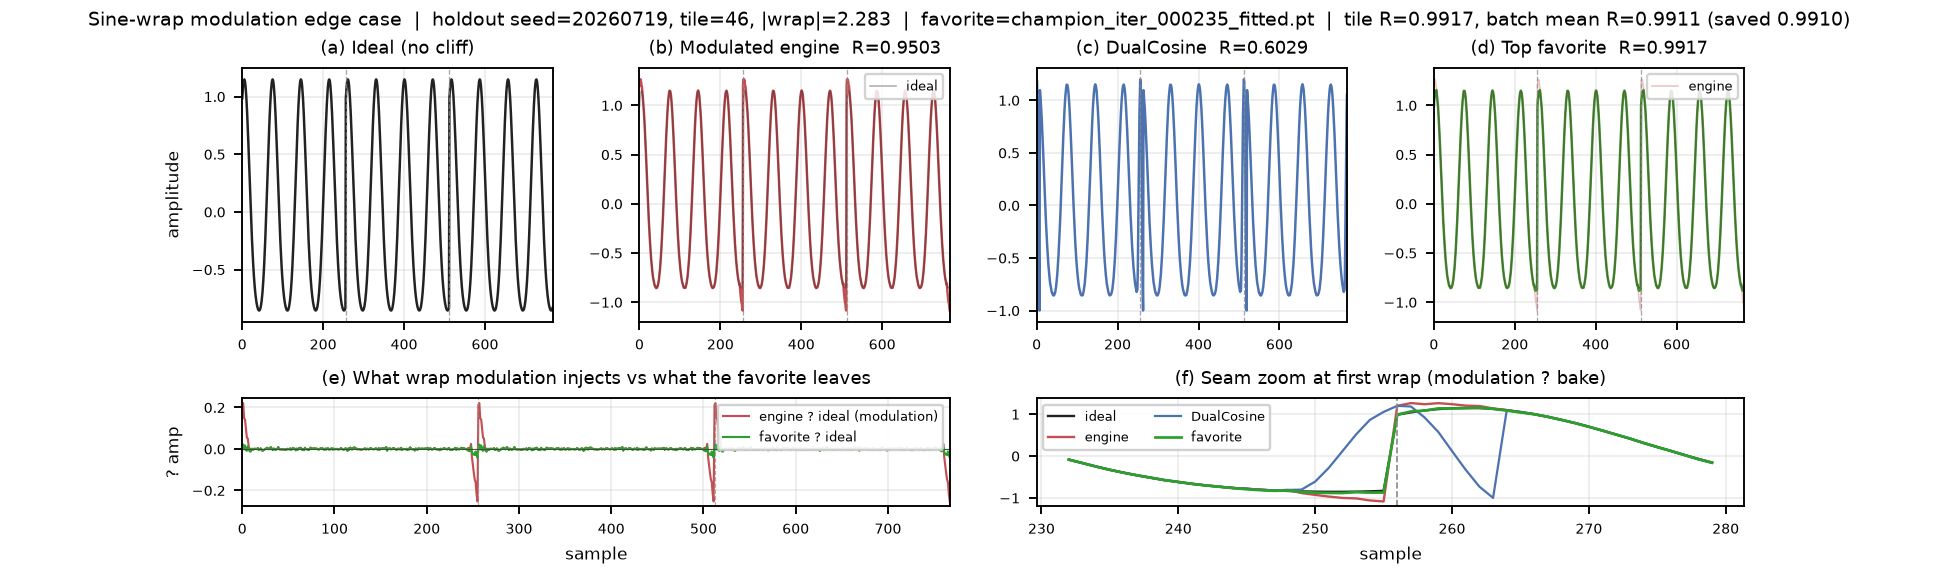
\includegraphics[width=\textwidth]{figures/fig_intro_sine_problem.png}
  \caption{Canonical holdout sine-wrap edge case (seed $20{,}260{,}719$, $L{=}256$, $N{=}16$ tiles, same tile across panels). (a)~Ideal sibling (cliff withheld). (b)~Engine with open-wrap cliff (ideal overlay). (c)~DualCosine bake. (d)~DenoiseOpt favorite bake. (e)--(f)~Modulation residual and seam zoom. Prolonged residual $R\in[0,1]$ (1~=~best) is printed per panel where scored.}
  \label{fig:intro-sine}
\end{figure*}

Classical virtual-analog practice already supplies seam-local tools.
Alias-free BLIT/BLEP-style synthesis~\cite{stilson1996}, PolyBLEP / fractional-delay antialiasing~\cite{nam2009polyblep}, and BLAMP corner corrections~\cite{esqueda2016blamp} reduce wrap and geometric discontinuity energy in-band.
Those operators act locally.
They leave open which bake parameters and which residual cell, if any, minimize prolonged tiled error against a no-cliff ideal.
Label-free restoration work such as Noise2Noise shows that useful reconstructors can be ranked without paired clean targets when the evaluation geometry is explicit~\cite{lehtinen2018}.
Speech-domain Noise2Noise denoisers extend that idea to audio waveforms~\cite{kashyap2021n2n}.
Mixture-invariant unsupervised separation likewise avoids paired clean stems for ranking~\cite{wisdom2020}.
On the search side, NAS surveys~\cite{elsken2019}, RL controllers~\cite{zoph2017nas,pham2018}, aging evolution~\cite{real2017large,real2019}, population-based hyperparameter schedules~\cite{jaderberg2017}, CMA-ES tutorials~\cite{hansen2016cmaes}, and evolution-guided policy gradients~\cite{khadka2018} motivate a hybrid outer loop: GA for population diversity, PPO for discrete architecture edits~\cite{schulman2017}, and PBT-style exploit--mutate on elites.
Platform-aware and progressive NAS add compute-aware search priors~\cite{tan2019mnasnet,liu2018pnas}.
MoE soft gates suggest routing among heterogeneous tiny cells under one residual score~\cite{shazeer2017}.
Waveform separation nets (Wave-U-Net, Conv-TasNet, dual-path RNN, SepFormer) and audio DL surveys inform the searchable cell family at bake-scale width~\cite{stoller2018,macartney2018,luo2019,luo2020dprnn,subakan2021,purwins2019,gong2021ast}, with U-Net / ResNet / attention primitives as block ancestors~\cite{ronneberger2015,he2016resnet,vaswani2017,jansson2017}.

The contribution is a meta-learning protocol for this periodic seam instance.
An outer RL+GA(+PBT) loop proposes bake-cell operator graphs and continuous bake parameters.
Each candidate is scored by prolonged residual $R\in[0,1]$ (1~=~best) between engine-baked multi-period audio and a procedural ideal tiling.
Paired studio-clean wavetables are not required for every trial.
Differentiable DSP modules~\cite{engel2020} place DualCosine / FIR / MLP seam ops in an interpretable stack.
Bayesian HPO~\cite{snoek2012} informs prior families that compete under the same $R$.
A CUDA overnight campaign (PPO+GA+PBT+NAS, depth and MoE biases) has passed a $5{,}000$-iteration clean gate with champion $R\approx 0.9909$ versus DualCosine $\approx 0.8166$ on the runner geometry.
The frozen canonical holdout and inference benches in Results are the measured evaluation matrices for this report.
We do not claim general speech or music enhancement SOTA.

\paragraph{Contributions.}
\begin{enumerate}
  \item \textbf{Problem framing.} Cast wavetable wrap discontinuity as cycle-local seam restoration under prolonged tiled evaluation, separating seam-local diagnostics from residual $R$.
  \item \textbf{Hybrid DenoiseOpt outer loop.} Specify RL+GA(+PBT) search over discrete operator graphs and continuous bake parameters, with named branches (GA crossover, PPO mutation, PBT exploit, MoE soft gates).
  \item \textbf{Formal residual protocol.} Define ideal-tile siblings, $R$ with range/perfect-match/monotone properties, and reimplementable Algorithms~\ref{alg:residual}--\ref{alg:hybrid}.
  \item \textbf{Open evaluation path.} Release companion code for the synthesizer engine and meta search, with frozen $5$k-gate figures and matched classical-vs-favorite benches.
\end{enumerate}

Section~\ref{sec:related_work} organizes related work by mechanism.
Sections~\ref{sec:methods}--\ref{sec:experiments} detail the residual objective and search protocol.
Results report the $5$k-gate freeze and inference benches.
